\documentclass{extbook}[14pt]
\usepackage{multicol, enumerate, enumitem, hyperref, color, soul, setspace, parskip, fancyhdr, amssymb, amsthm, amsmath, latexsym, units, mathtools}
\everymath{\displaystyle}
\usepackage[headsep=0.5cm,headheight=0cm, left=1 in,right= 1 in,top= 1 in,bottom= 1 in]{geometry}
\usepackage{dashrule}  % Package to use the command below to create lines between items
\newcommand{\litem}[1]{\item #1

\rule{\textwidth}{0.4pt}}
\pagestyle{fancy}
\lhead{}
\chead{Answer Key for Progress Quiz 6 Version A}
\rhead{}
\lfoot{1430-1829}
\cfoot{}
\rfoot{test}
\begin{document}
\textbf{This key should allow you to understand why you choose the option you did (beyond just getting a question right or wrong). \href{https://xronos.clas.ufl.edu/mac1105spring2020/courseDescriptionAndMisc/Exams/LearningFromResults}{More instructions on how to use this key can be found here}.}

\textbf{If you have a suggestion to make the keys better, \href{https://forms.gle/CZkbZmPbC9XALEE88}{please fill out the short survey here}.}

\textit{Note: This key is auto-generated and may contain issues and/or errors. The keys are reviewed after each exam to ensure grading is done accurately. If there are issues (like duplicate options), they are noted in the offline gradebook. The keys are a work-in-progress to give students as many resources to improve as possible.}

\rule{\textwidth}{0.4pt}

\begin{enumerate}\litem{
Construct the lowest-degree polynomial given the zeros below. Then, choose the intervals that contain the coefficients of the polynomial in the form $x^3+bx^2+cx+d$.
\[ 5 + 3 i \text{ and } 3 \]The solution is \( x^{3} -13 x^{2} +64 x -102 \), which is option B.\begin{enumerate}[label=\Alph*.]
\item \( b \in [10, 18], c \in [62.11, 64.76], \text{ and } d \in [101, 106.3] \)

$x^{3} +13 x^{2} +64 x + 102$, which corresponds to multiplying out $(x-(5 + 3 i))(x-(5 - 3 i))(x + 3)$.
\item \( b \in [-21, -5], c \in [62.11, 64.76], \text{ and } d \in [-105.1, -100.1] \)

* $x^{3} -13 x^{2} +64 x -102$, which is the correct option.
\item \( b \in [1, 3], c \in [-8.79, -7.83], \text{ and } d \in [11.8, 17] \)

$x^{3} + x^{2} -8 x + 15$, which corresponds to multiplying out $(x -5)(x -3)$.
\item \( b \in [1, 3], c \in [-7.39, -4.76], \text{ and } d \in [5.2, 9.5] \)

$x^{3} + x^{2} -6 x + 9$, which corresponds to multiplying out $(x -3)(x -3)$.
\item \( \text{None of the above.} \)

This corresponds to making an unanticipated error or not understanding how to use nonreal complex numbers to create the lowest-degree polynomial. If you chose this and are not sure what you did wrong, please contact the coordinator for help.
\end{enumerate}

\textbf{General Comment:} Remember that the conjugate of $a+bi$ is $a-bi$. Since these zeros always come in pairs, we need to multiply out $(x-(5 + 3 i))(x-(5 - 3 i))(x-(3))$.
}
\litem{
Describe the end behavior of the polynomial below.
\[ f(x) = 8(x - 6)^{4}(x + 6)^{9}(x + 9)^{4}(x - 9)^{5} \]The solution is the graph below, which is option C.
\begin{center}
    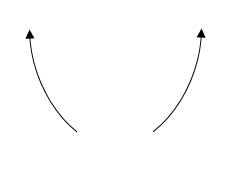
\includegraphics[width=0.3\textwidth]{../Figures/polyEndBehaviorCopyCA.png}
\end{center}\begin{enumerate}[label=\Alph*.]
\begin{multicols}{2}
\item 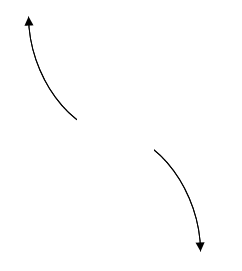
\includegraphics[width = 0.3\textwidth]{../Figures/polyEndBehaviorCopyAA.png}
\item 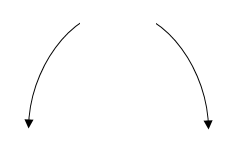
\includegraphics[width = 0.3\textwidth]{../Figures/polyEndBehaviorCopyBA.png}
\item 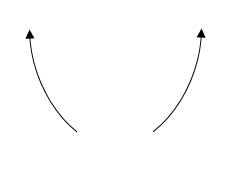
\includegraphics[width = 0.3\textwidth]{../Figures/polyEndBehaviorCopyCA.png}
\item 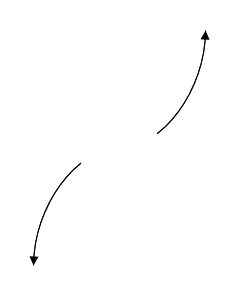
\includegraphics[width = 0.3\textwidth]{../Figures/polyEndBehaviorCopyDA.png}
\end{multicols}\item None of the above.\end{enumerate}
\textbf{General Comment:} Remember that end behavior is determined by the leading coefficient AND whether the \textbf{sum} of the multiplicities is positive or negative.
}
\litem{
Describe the zero behavior of the zero $x = 7$ of the polynomial below.
\[ f(x) = 9(x + 7)^{8}(x - 7)^{11}(x - 3)^{7}(x + 3)^{10} \]The solution is the graph below, which is option D.
\begin{center}
    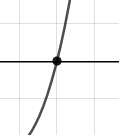
\includegraphics[width=0.3\textwidth]{../Figures/polyZeroBehaviorDA.png}
\end{center}\begin{enumerate}[label=\Alph*.]
\begin{multicols}{2}
\item 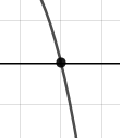
\includegraphics[width = 0.3\textwidth]{../Figures/polyZeroBehaviorAA.png}
\item 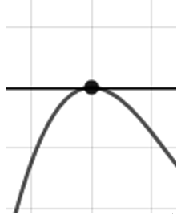
\includegraphics[width = 0.3\textwidth]{../Figures/polyZeroBehaviorBA.png}
\item 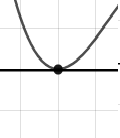
\includegraphics[width = 0.3\textwidth]{../Figures/polyZeroBehaviorCA.png}
\item 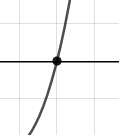
\includegraphics[width = 0.3\textwidth]{../Figures/polyZeroBehaviorDA.png}
\end{multicols}\item None of the above.\end{enumerate}
\textbf{General Comment:} You will need to sketch the entire graph, then zoom in on the zero the question asks about.
}
\litem{
Construct the lowest-degree polynomial given the zeros below. Then, choose the intervals that contain the coefficients of the polynomial in the form $ax^3+bx^2+cx+d$.
\[ \frac{-5}{3}, -3, \text{ and } \frac{5}{4} \]The solution is \( 12x^{3} +41 x^{2} -10 x -75 \), which is option D.\begin{enumerate}[label=\Alph*.]
\item \( a \in [12, 15], b \in [-43, -40], c \in [-16, -2], \text{ and } d \in [71, 81] \)

$12x^{3} -41 x^{2} -10 x + 75$, which corresponds to multiplying out $(3x -5)(x -3)(4x + 5)$.
\item \( a \in [12, 15], b \in [37, 49], c \in [-16, -2], \text{ and } d \in [71, 81] \)

$12x^{3} +41 x^{2} -10 x + 75$, which corresponds to multiplying everything correctly except the constant term.
\item \( a \in [12, 15], b \in [-2, 3], c \in [-84, -79], \text{ and } d \in [71, 81] \)

$12x^{3} + x^{2} -80 x + 75$, which corresponds to multiplying out $(3x -5)(x + 3)(4x -5)$.
\item \( a \in [12, 15], b \in [37, 49], c \in [-16, -2], \text{ and } d \in [-78, -73] \)

* $12x^{3} +41 x^{2} -10 x -75$, which is the correct option.
\item \( a \in [12, 15], b \in [-85, -66], c \in [126, 135], \text{ and } d \in [-78, -73] \)

$12x^{3} -71 x^{2} +130 x -75$, which corresponds to multiplying out $(3x -5)(x -3)(4x -5)$.
\end{enumerate}

\textbf{General Comment:} To construct the lowest-degree polynomial, you want to multiply out $(3x + 5)(x + 3)(4x -5)$
}
\litem{
Construct the lowest-degree polynomial given the zeros below. Then, choose the intervals that contain the coefficients of the polynomial in the form $ax^3+bx^2+cx+d$.
\[ \frac{-6}{5}, \frac{-4}{3}, \text{ and } -3 \]The solution is \( 15x^{3} +83 x^{2} +138 x + 72 \), which is option E.\begin{enumerate}[label=\Alph*.]
\item \( a \in [13, 21], b \in [76, 90], c \in [133, 140], \text{ and } d \in [-75, -70] \)

$15x^{3} +83 x^{2} +138 x -72$, which corresponds to multiplying everything correctly except the constant term.
\item \( a \in [13, 21], b \in [42, 53], c \in [-19, -16], \text{ and } d \in [-75, -70] \)

$15x^{3} +47 x^{2} -18 x -72$, which corresponds to multiplying out $(5x -6)(3x + 4)(x + 3)$.
\item \( a \in [13, 21], b \in [3, 8], c \in [-91, -85], \text{ and } d \in [66, 76] \)

$15x^{3} +7 x^{2} -90 x + 72$, which corresponds to multiplying out $(5x -6)(3x -4)(x + 3)$.
\item \( a \in [13, 21], b \in [-84, -78], c \in [133, 140], \text{ and } d \in [-75, -70] \)

$15x^{3} -83 x^{2} +138 x -72$, which corresponds to multiplying out $(5x -6)(3x -4)(x -3)$.
\item \( a \in [13, 21], b \in [76, 90], c \in [133, 140], \text{ and } d \in [66, 76] \)

* $15x^{3} +83 x^{2} +138 x + 72$, which is the correct option.
\end{enumerate}

\textbf{General Comment:} To construct the lowest-degree polynomial, you want to multiply out $(5x + 6)(3x + 4)(x + 3)$
}
\litem{
Which of the following equations \textit{could} be of the graph presented below?

\begin{center}
    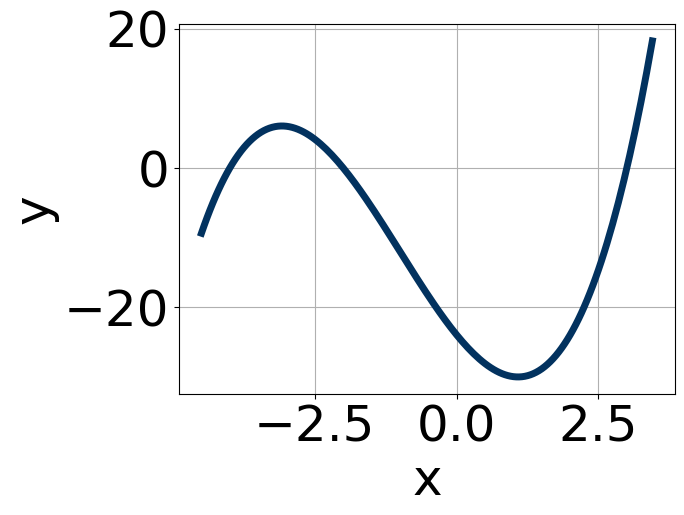
\includegraphics[width=0.5\textwidth]{../Figures/polyGraphToFunctionCopyA.png}
\end{center}


The solution is \( 20(x + 4)^{9} (x - 1)^{11} (x + 3)^{7} \), which is option E.\begin{enumerate}[label=\Alph*.]
\item \( -11(x + 4)^{7} (x - 1)^{7} (x + 3)^{11} \)

This corresponds to the leading coefficient being the opposite value than it should be.
\item \( -3(x + 4)^{8} (x - 1)^{11} (x + 3)^{11} \)

The factor $(x + 4)$ should have an odd power and the leading coefficient should be the opposite sign.
\item \( 18(x + 4)^{8} (x - 1)^{7} (x + 3)^{5} \)

The factor $-4$ should have been an odd power.
\item \( 6(x + 4)^{4} (x - 1)^{10} (x + 3)^{5} \)

The factors $-4$ and $1$ have have been odd power.
\item \( 20(x + 4)^{9} (x - 1)^{11} (x + 3)^{7} \)

* This is the correct option.
\end{enumerate}

\textbf{General Comment:} General Comments: Draw the x-axis to determine which zeros are touching (and so have even multiplicity) or cross (and have odd multiplicity).
}
\litem{
Which of the following equations \textit{could} be of the graph presented below?

\begin{center}
    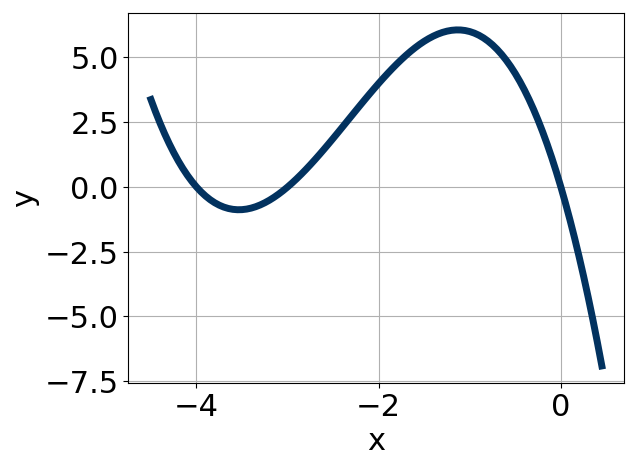
\includegraphics[width=0.5\textwidth]{../Figures/polyGraphToFunctionA.png}
\end{center}


The solution is \( -11(x + 4)^{6} (x - 3)^{10} (x + 2)^{5} \), which is option B.\begin{enumerate}[label=\Alph*.]
\item \( -5(x + 4)^{10} (x - 3)^{11} (x + 2)^{7} \)

The factor $(x - 3)$ should have an even power.
\item \( -11(x + 4)^{6} (x - 3)^{10} (x + 2)^{5} \)

* This is the correct option.
\item \( 9(x + 4)^{6} (x - 3)^{10} (x + 2)^{11} \)

This corresponds to the leading coefficient being the opposite value than it should be.
\item \( -19(x + 4)^{4} (x - 3)^{9} (x + 2)^{6} \)

The factor $(x - 3)$ should have an even power and the factor $(x + 2)$ should have an odd power.
\item \( 19(x + 4)^{4} (x - 3)^{8} (x + 2)^{4} \)

The factor $(x + 2)$ should have an odd power and the leading coefficient should be the opposite sign.
\end{enumerate}

\textbf{General Comment:} General Comments: Draw the x-axis to determine which zeros are touching (and so have even multiplicity) or cross (and have odd multiplicity).
}
\litem{
Describe the zero behavior of the zero $x = -7$ of the polynomial below.
\[ f(x) = -8(x - 7)^{8}(x + 7)^{13}(x - 9)^{4}(x + 9)^{7} \]The solution is the graph below, which is option A.
\begin{center}
    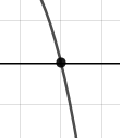
\includegraphics[width=0.3\textwidth]{../Figures/polyZeroBehaviorCopyAA.png}
\end{center}\begin{enumerate}[label=\Alph*.]
\begin{multicols}{2}
\item 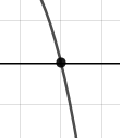
\includegraphics[width = 0.3\textwidth]{../Figures/polyZeroBehaviorCopyAA.png}
\item 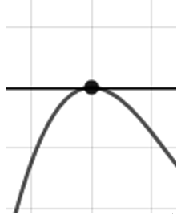
\includegraphics[width = 0.3\textwidth]{../Figures/polyZeroBehaviorCopyBA.png}
\item 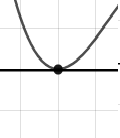
\includegraphics[width = 0.3\textwidth]{../Figures/polyZeroBehaviorCopyCA.png}
\item 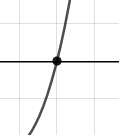
\includegraphics[width = 0.3\textwidth]{../Figures/polyZeroBehaviorCopyDA.png}
\end{multicols}\item None of the above.\end{enumerate}
\textbf{General Comment:} You will need to sketch the entire graph, then zoom in on the zero the question asks about.
}
\litem{
Construct the lowest-degree polynomial given the zeros below. Then, choose the intervals that contain the coefficients of the polynomial in the form $x^3+bx^2+cx+d$.
\[ -5 + 3 i \text{ and } 1 \]The solution is \( x^{3} +9 x^{2} +24 x -34 \), which is option A.\begin{enumerate}[label=\Alph*.]
\item \( b \in [4, 10], c \in [22, 26], \text{ and } d \in [-38, -33] \)

* $x^{3} +9 x^{2} +24 x -34$, which is the correct option.
\item \( b \in [-16, -7], c \in [22, 26], \text{ and } d \in [27, 36] \)

$x^{3} -9 x^{2} +24 x + 34$, which corresponds to multiplying out $(x-(-5 + 3 i))(x-(-5 - 3 i))(x + 1)$.
\item \( b \in [-4, 5], c \in [1, 6], \text{ and } d \in [-12, -3] \)

$x^{3} + x^{2} +4 x -5$, which corresponds to multiplying out $(x + 5)(x -1)$.
\item \( b \in [-4, 5], c \in [-4, 0], \text{ and } d \in [2, 4] \)

$x^{3} + x^{2} -4 x + 3$, which corresponds to multiplying out $(x -3)(x -1)$.
\item \( \text{None of the above.} \)

This corresponds to making an unanticipated error or not understanding how to use nonreal complex numbers to create the lowest-degree polynomial. If you chose this and are not sure what you did wrong, please contact the coordinator for help.
\end{enumerate}

\textbf{General Comment:} Remember that the conjugate of $a+bi$ is $a-bi$. Since these zeros always come in pairs, we need to multiply out $(x-(-5 + 3 i))(x-(-5 - 3 i))(x-(1))$.
}
\litem{
Describe the end behavior of the polynomial below.
\[ f(x) = -4(x + 4)^{3}(x - 4)^{6}(x - 5)^{2}(x + 5)^{3} \]The solution is the graph below, which is option B.
\begin{center}
    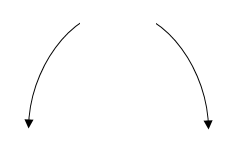
\includegraphics[width=0.3\textwidth]{../Figures/polyEndBehaviorBA.png}
\end{center}\begin{enumerate}[label=\Alph*.]
\begin{multicols}{2}
\item 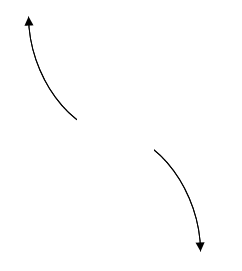
\includegraphics[width = 0.3\textwidth]{../Figures/polyEndBehaviorAA.png}
\item 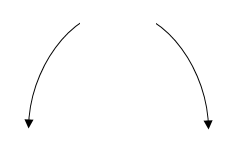
\includegraphics[width = 0.3\textwidth]{../Figures/polyEndBehaviorBA.png}
\item 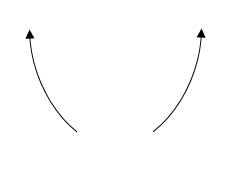
\includegraphics[width = 0.3\textwidth]{../Figures/polyEndBehaviorCA.png}
\item 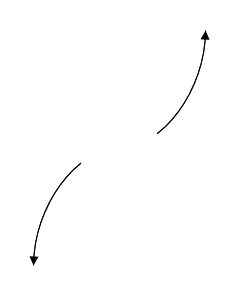
\includegraphics[width = 0.3\textwidth]{../Figures/polyEndBehaviorDA.png}
\end{multicols}\item None of the above.\end{enumerate}
\textbf{General Comment:} Remember that end behavior is determined by the leading coefficient AND whether the \textbf{sum} of the multiplicities is positive or negative.
}
\end{enumerate}

\end{document}